%!TEX root = ../../../report.tex
\section{Environment creation} % (fold)
\label{sec:environment_creation}
Besides the robot, other elements can be added to the simulated world.
From the Gazebo database, other robot models or parts (as a beer or a brick) can be inserted and used for any kind of experiments.

In the framework we provide an extra tool: a rotational robot holder.
This is inspired from the Dacbot simulation in LPZ Robots, is fully parametric and reduces the degrees of freedom of the robot so more specific experiments can be carried out.

\begin{figure}[hb!]
  \centering
  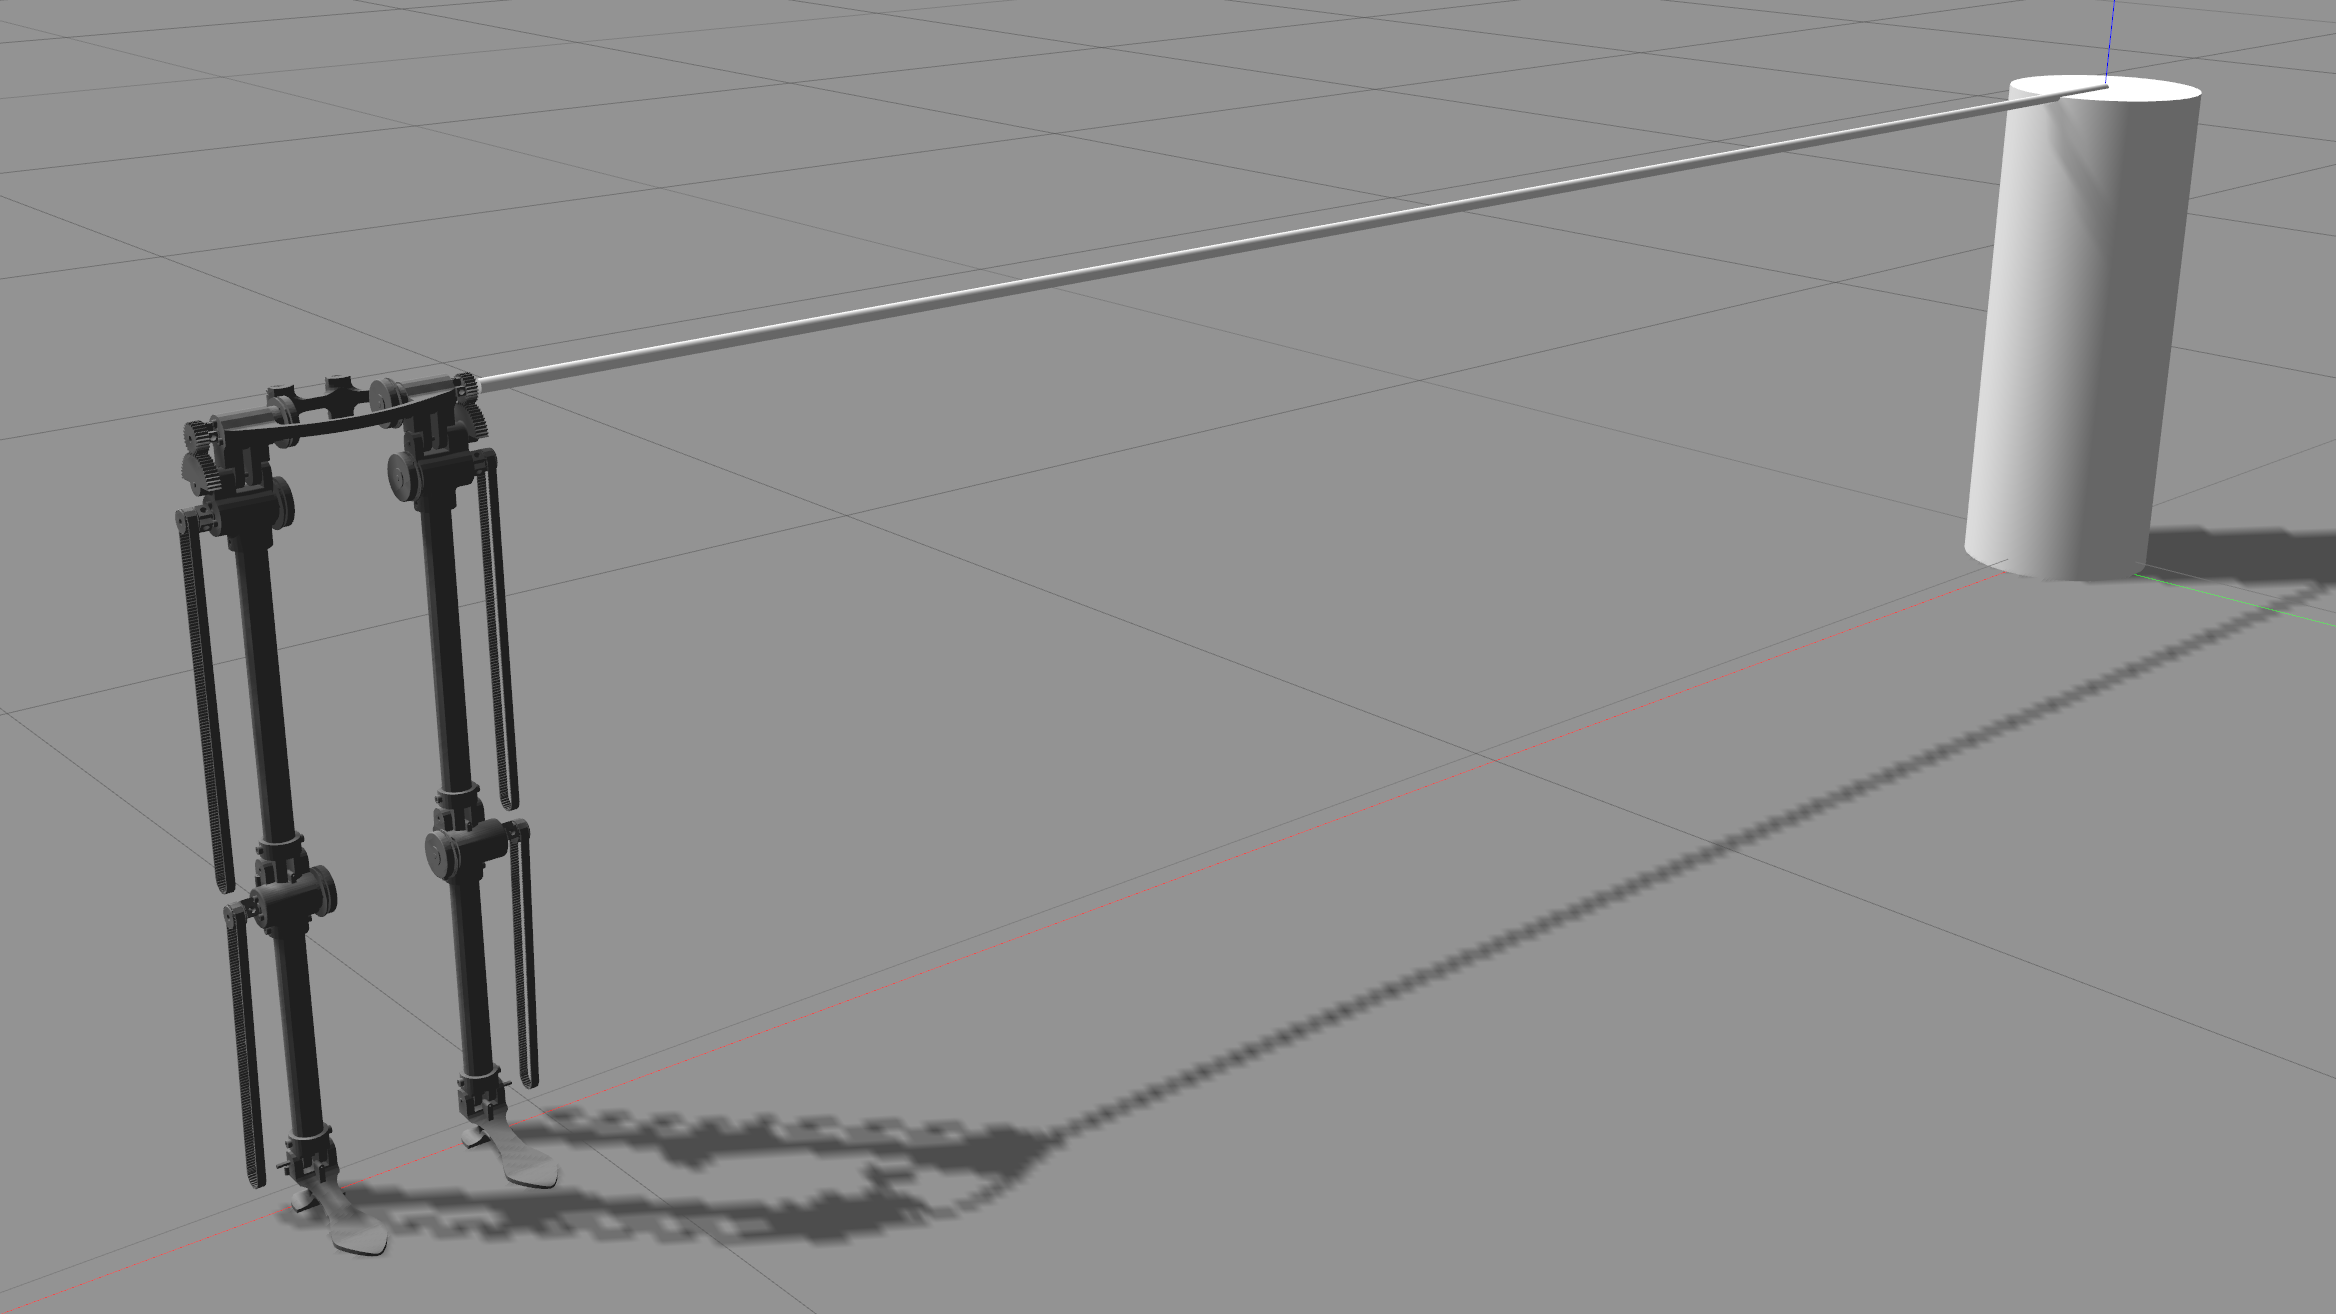
\includegraphics[width=0.75\linewidth]{figures/gazebo_rotational_holder}
  \caption{Rotational robot holder and robot}
  \label{fig:rotational_robot_holder}
\end{figure}
% section environment_creation (end)